\documentclass[10pt]{beamer}

\useinnertheme[shadow=true]{rounded}
\useoutertheme{infolines}
\usecolortheme{whale}
\usecolortheme[RGB={245,128,37}]{structure}

\definecolor{bold}{RGB}{245,128,37}

\newcommand{\drawdownarrow}{\centering \vspace{0.05in}  {\LARGE $\downarrow$}  \vspace{0.05in}}
\DeclareMathOperator*{\argmin}{arg\,min}

\makeatletter
\setbeamertemplate{footline}
{
  \leavevmode%
  \hbox{%
  \begin{beamercolorbox}[wd=.333333\paperwidth,ht=2.25ex,dp=1ex,center]{author in head/foot}%
    \usebeamerfont{author in head/foot}\insertshortauthor~~\beamer@ifempty{\insertshortinstitute}{}{(\insertshortinstitute)}
  \end{beamercolorbox}%
  \begin{beamercolorbox}[wd=.333333\paperwidth,ht=2.25ex,dp=1ex,center]{title in head/foot}%
    \usebeamerfont{title in head/foot}\insertshorttitle
  \end{beamercolorbox}%
  \begin{beamercolorbox}[wd=.333333\paperwidth,ht=2.25ex,dp=1ex,right]{date in head/foot}%
    \usebeamerfont{date in head/foot}\insertshortdate{}\hspace*{8em}
    \insertframenumber\hspace*{2ex} 
  \end{beamercolorbox}}%
  \vskip0pt%
}
\makeatother
  
\usepackage{ragged2e}
%\usepackage{setspace}

\usepackage{forloop}
\usepackage[percent]{overpic}

\usepackage{extarrows}
\usepackage{tikz}
\usetikzlibrary{calc}
\usetikzlibrary{arrows}
\usetikzlibrary{decorations.markings}
\usetikzlibrary{positioning}

\usepackage{movie15}

\usepackage{animate}
\usepackage{amssymb}
\usepackage{color}
\beamertemplatenavigationsymbolsempty

\hyphenpenalty 10000
\exhyphenpenalty 10000
\widowpenalty 10000
\clubpenalty 10000

\usepackage[firstinits=true,style=verbose,maxnames=6,backend=bibtex]{biblatex}
\renewbibmacro{in:}{}
\bibliography{../../references/references}
\setbeamercolor{bibliography item}{use=normal text,fg=black}
\setbeamercolor*{bibliography entry title}{use=normal text,fg=black}
\setbeamercolor*{bibliography entry author}{use=normal text,fg=black}
\setbeamercolor*{bibliography entry journal}{use=normal text,fg=black}
\setbeamercolor*{bibliography entry note}{use=normal text,fg=black}

\DeclareCiteCommand{\footcite}{}{%
    \footnote{\printnames[author]{author}, \printfield{journaltitle}, \printfield{year}}} {\textsuperscript{,}}{}%

\DeclareCiteCommand{\footcitetext}{}{%
    \footnotetext{\printnames[author]{author}, \printfield{journaltitle}, \printfield{year}}} {\textsuperscript{,}}{}%    
    

\DeclareCiteCommand{\cite}{}{%
    \printnames[author]{author}, \printfield{journaltitle}, \printfield{year}} {;}{}%

\let\oldfootnotesize\footnotesize
\renewcommand*{\footnotesize}{\oldfootnotesize\tiny}


	

\graphicspath{ {images/} }

\title[Registration and Temporal Ordering of Images]{Registration and Temporal Ordering of Images in Studies of Biological Development}

\author[C. Dsilva]{{\bf Carmeline~Dsilva}\inst{1},  Bomyi~Lim\inst{1}, Stanislav~Shvartsman\inst{1,2}, and Ioannis~Kevrekidis\inst{1,3}}
\institute[Princeton]{
  \inst{1}Department of Chemical and Biological Engineering\\
  \inst{2}Lewis-Sigler Institute for Integrative Genomics \\
  \inst{3}Program in Applied and Computational Mathematics \\
  Princeton University, Princeton, NJ 
  \\[1ex]
  \texttt{cdsilva@princeton.edu}
}
\date[April 2014]{14 April 2014}

\begin{document}

\begin{frame}[plain]
  \titlepage
  \hfill
  
\includegraphics[width=1in]{PUsig2}
\end{frame}

\begin{frame}{Reconstructing Dynamics from Snapshots}

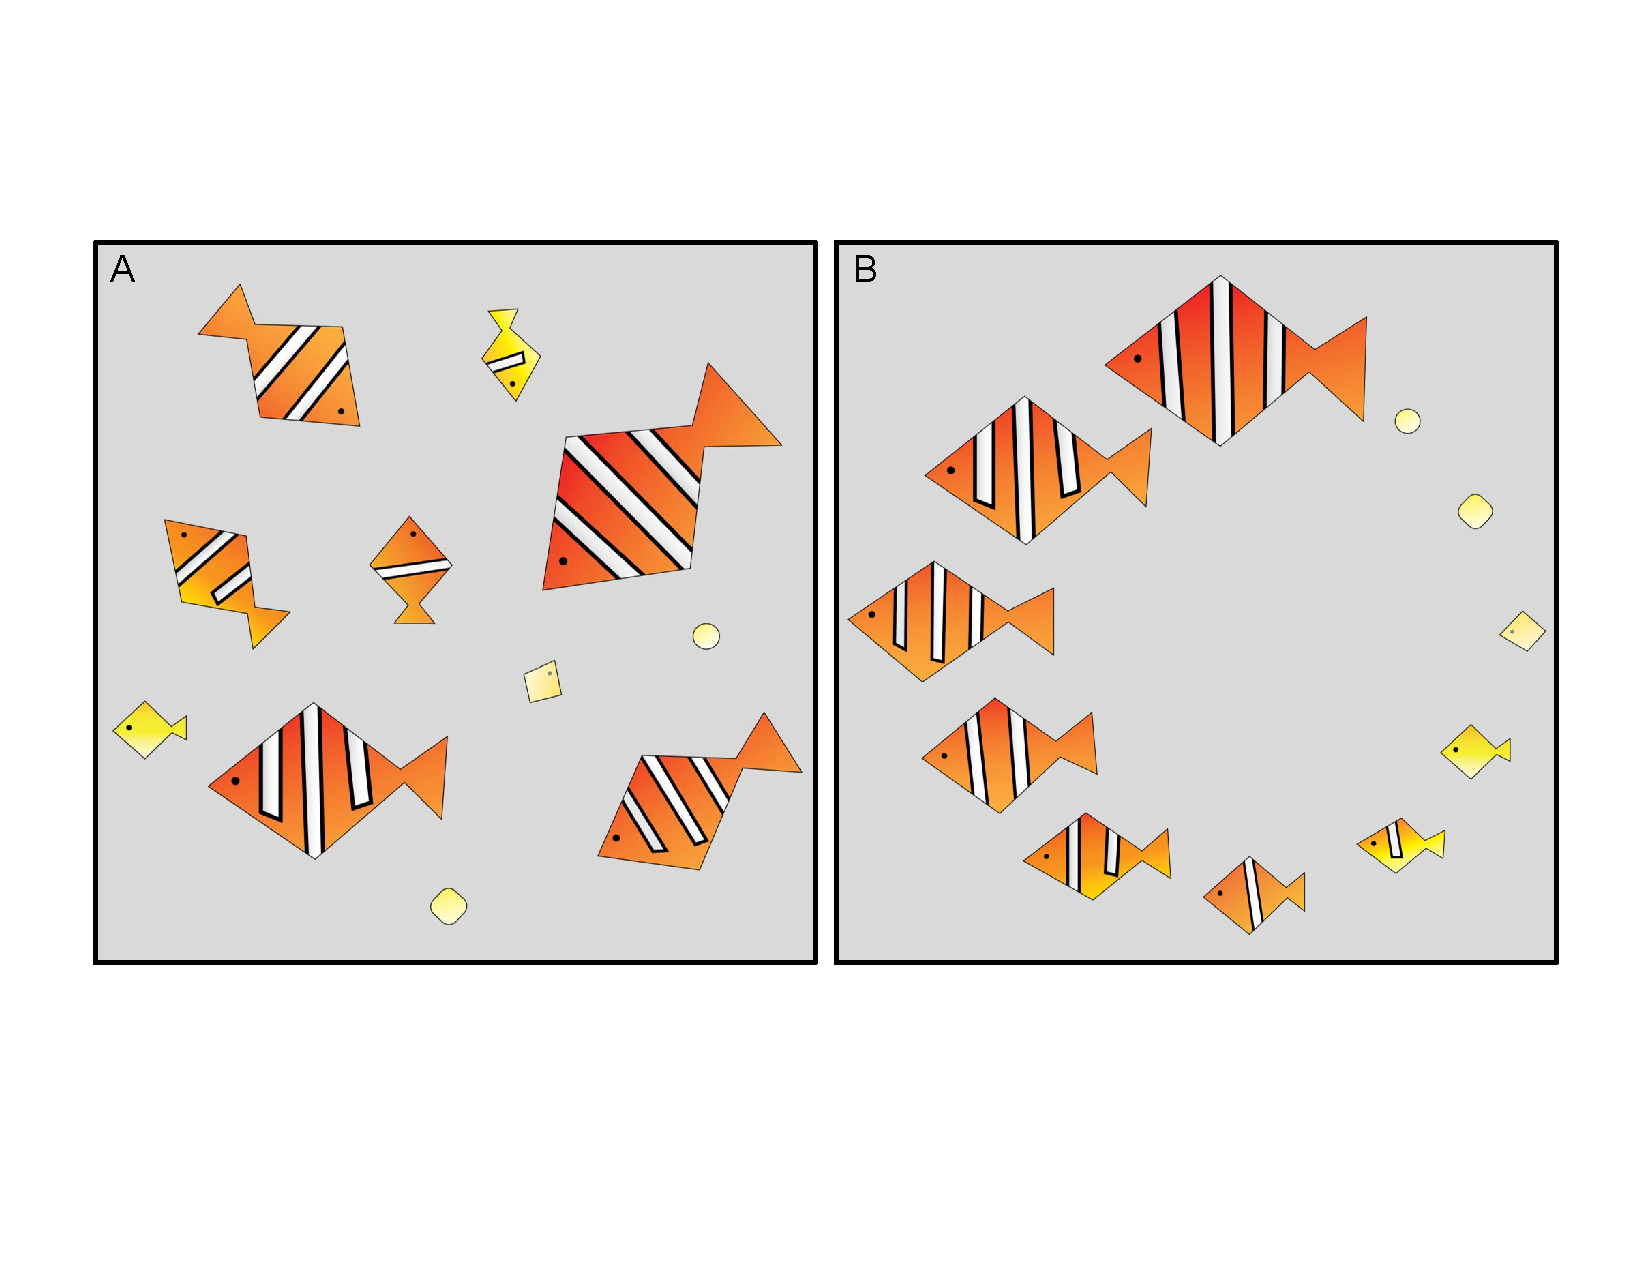
\includegraphics[width=0.5\textwidth]{fig1}

\end{frame}

\section{Experimental Setup}

\begin{frame}{{\em Drosophila}: Our Model System}

\end{frame}

\begin{frame}{Data Collection}

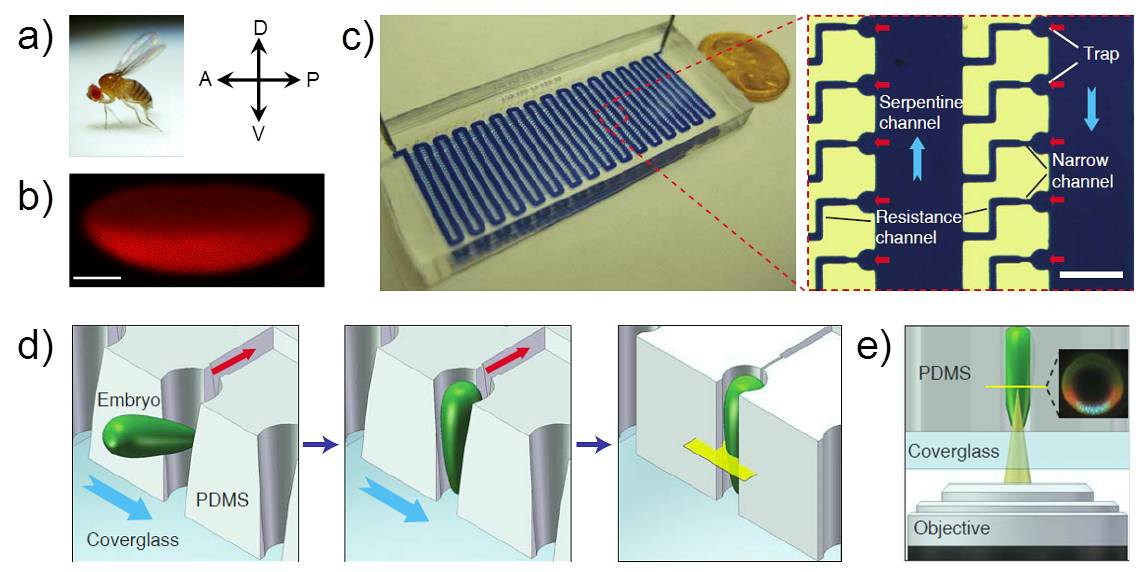
\includegraphics[width=0.7\textwidth]{drosophila_imaging_setup}

\end{frame}

\begin{frame}{A Typical Data Set}

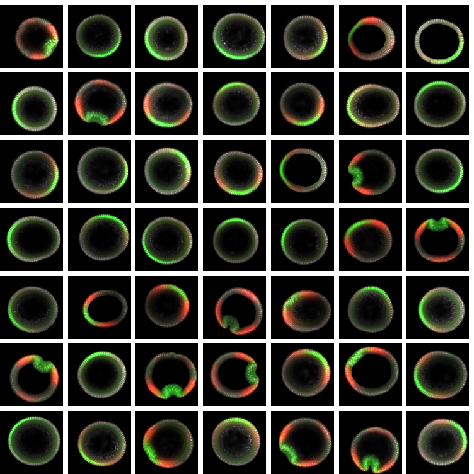
\includegraphics[width=0.5\textwidth]{fig2a}

\end{frame}

\section{Mathematical Methods}

\begin{frame}{Outline of Mathematical Methods}

\begin{itemize}

\item Image registration using angular synchronization \footcite{singer2011angular}

\item Temporal ordering using diffusion maps \footcite{coifman2005geometric}

\item Simultaneous registration and ordering using vector diffusion maps \footcite{singer2012vector}

\end{itemize}
\end{frame}

\begin{frame}{Image Registration: Angular Synchronization}

\end{frame}

\begin{frame}{Temporal Ordering: Diffusion Maps}

\end{frame}

\begin{frame}{Combined: Vector Diffusion Maps}

\end{frame}

\section{Future Work}

\begin{frame}{Future Directions}

\begin{itemize}
\item Make a smooth movie from images
\item Look at images over a larger dynamical range, where the embryos change shape and morph
\item Look at images where texture-like features (i.e., number of nuclei) are important
\end{itemize}
\end{frame}

\end{document}
